\section*{Use Case Model}
Two scenarios have been taken into account, where the user gets lost in the museum, and the user wants to explore the museum. When a user is lost, they need to enter their destination where the app will receive their current location, and find the quickest route from the user's current position. The user follows that navigation until they arrive at their destination. For the exploration, the app will show the details where user know what they going to see in the museum.

\subsection*{Activity Model}
This is based on the back-end of the application for example when the user searches about the museum, this history saved in the server where if the user wants to go to the same place then they can use our function called past visit.

\section*{User \& Acceptance Stories}
This will describe what will be achieved once the application is ready to be used by the user. A diagram has been created based on different scenarios where it can be found if the application has achieved the user needs. 

\begin{figure}[H]
    \centering
    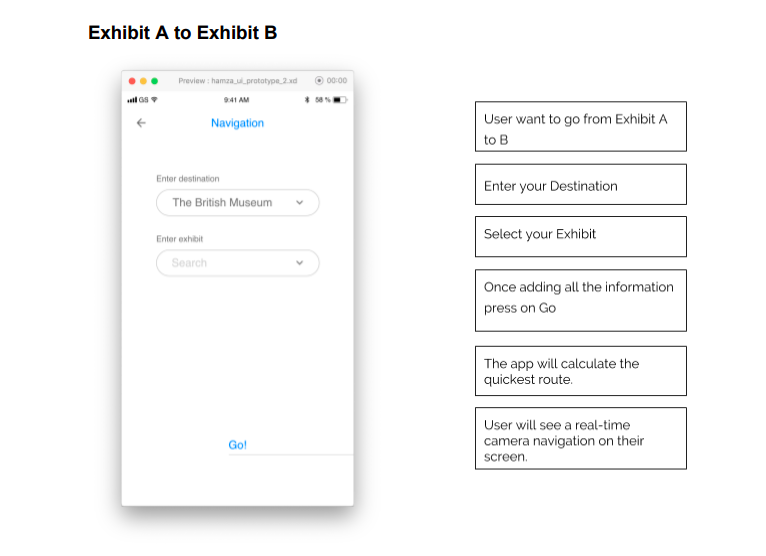
\includegraphics[width=\textwidth]
    {userstories/userstory_aTob.png}
    \caption{Going from point A to point B}
    \label{fig:AtoB}
\end{figure}

\begin{figure}[H]
    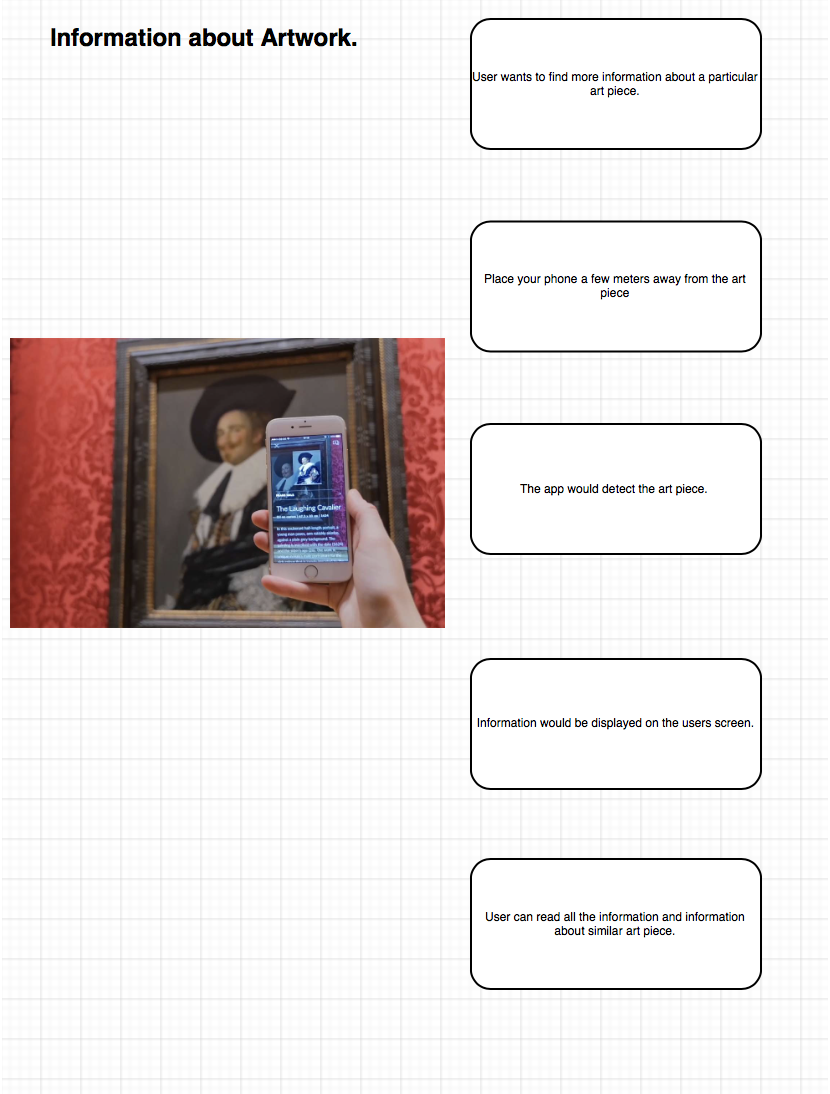
\includegraphics[width=\textwidth]
    {userstories/userstory_info.png}
    \caption{Getting information from exhibition}
    \label{fig:infofromexhibit}
\end{figure}

\begin{figure}[H]
    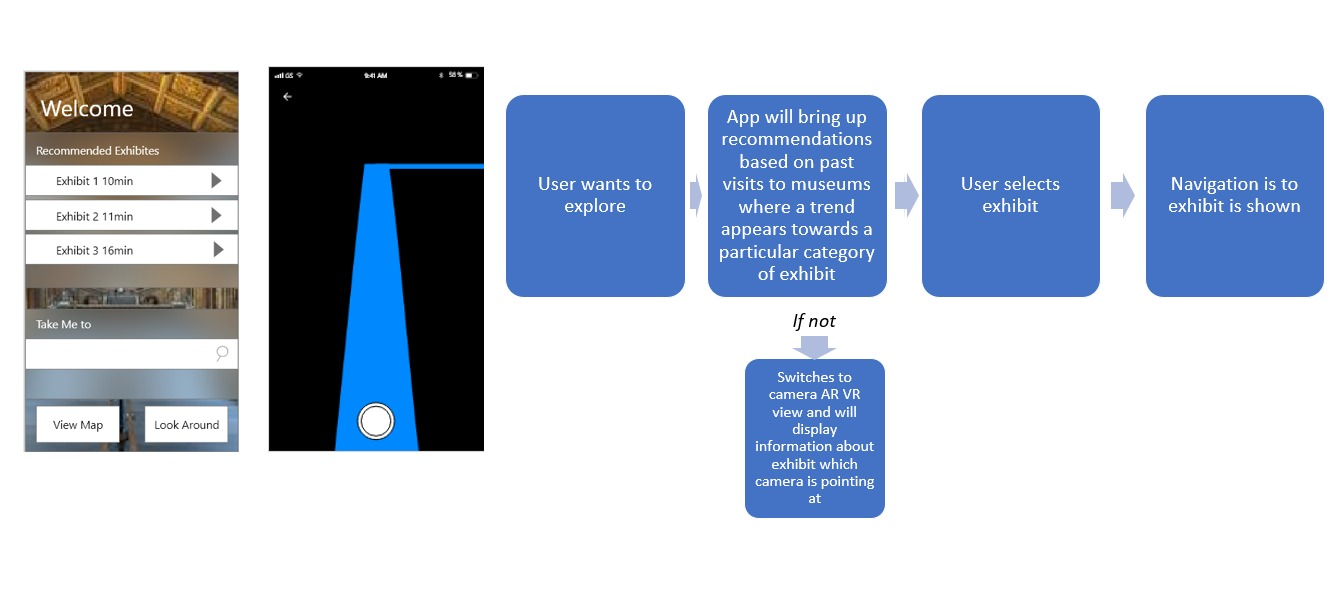
\includegraphics[width=\textwidth]
    {userstories/userstory_explore.jpeg}
    \caption{Exploring the museum}
    \label{fig:exploring}
\end{figure}
